\documentclass{article}
\usepackage{amsmath}
\usepackage{graphicx}

\begin{document}

\section*{Graph Connectivity and Eigenvalues}
\subsection*{Definition}
In graph theory, connectivity refers to a measure of how connected or interconnected a graph is. It quantifies the ability to travel or navigate between vertices (nodes) in a graph. The connectivity of a graph is important in understanding its structural properties and determining how easily information or resources can flow through the network represented by the graph.

\textbf{Strong Connectivity:}
A directed graph is strongly connected if there is a directed path between any two vertices in the graph. In other words, it is possible to reach any vertex from any other vertex in the graph.

\textbf{Weak Connectivity:}
A directed graph is weakly connected if replacing all the directed edges with undirected edges produces a connected undirected graph. In other words, it is possible to reach any vertex from any other vertex when considering the graph as undirected.

\subsection*{Graph Connectivity}

The connectivity of a graph can be determined using the Laplacian matrix. By calculating the eigenvalues of the Laplacian matrix and examining the second smallest eigenvalue, you can determine whether the graph is disconnected or has multiple connected components.

\textbf{Theorem:} The second smallest eigenvalue $\lambda_2$ tells you about the connectivity of the graph. If the graph has two disconnected components, $\lambda_2 = 0$. And if $\lambda_2$ is small, this suggests the graph is nearly disconnected, with two components that are not very connected to each other.

\textbf{Proof:}

\begin{enumerate}
  \item Let $v_1, v_2, \ldots, v_k$ be $k$ eigenvectors corresponding to the eigenvalue $0$, where $k$ is the multiplicity of $0$ as an eigenvalue.
  \item Consider the vector $x = v_1 + v_2 + \ldots + v_k$. Since $L$ is a linear operator, we have $Lx = Lv_1 + Lv_2 + \ldots + Lv_k = 0 + 0 + \ldots + 0 = 0$.
  \item Now, suppose the graph $G$ has $m$ connected components, where $m \leq k$.
  \item Let $C_1, C_2, \ldots, C_m$ be the $m$ connected components of $G$. Each connected component $C_i$ has its corresponding eigenvector $v_i$, where $1 \leq i \leq m$. Note that each $v_i$ has entries corresponding to vertices only in the connected component $C_i$, and all other entries are $0$.
  \item Therefore, when we sum up all the eigenvectors $v_1, v_2, \ldots, v_k$, we get $x = v_1 + v_2 + \ldots + v_k$, which has entries corresponding to vertices in all connected components $C_i$, and all other entries are $0$.
  \item Since $Lx = 0$, we have $Lx = L(v_1 + v_2 + \ldots + v_k) = Lv_1 + Lv_2 + \ldots + Lv_k = 0$. But since each $Lv_1, Lv_2, \ldots, Lv_k$ corresponds to a connected component $C_i$ and all other entries are $0$, we can rewrite the equation as $Lx = L(v_1 + v_2 + \ldots + v_k) = L(v_1) + L(v_2) + \ldots + L(v_k) = 0$.
  \item This implies that for each connected component $C_i$, we have $L(v_i) = 0$. In other words, each connected component has an eigenvector corresponding to the eigenvalue $0$.
  \item Since $m$ is the number of connected components and $m \leq k$, we conclude that the multiplicity of $0$ as an eigenvalue of $L$ is equal to the number of connected components in the graph.
\end{enumerate}

Hence, if the second smallest eigenvalue of the Laplacian matrix is $0$ (i.e., $\lambda_2 = 0$), it implies that the graph is disconnected.
\section*{Example}
\subsection*{Let us see this graph:}
\begin{figure}[h]
    \centering
    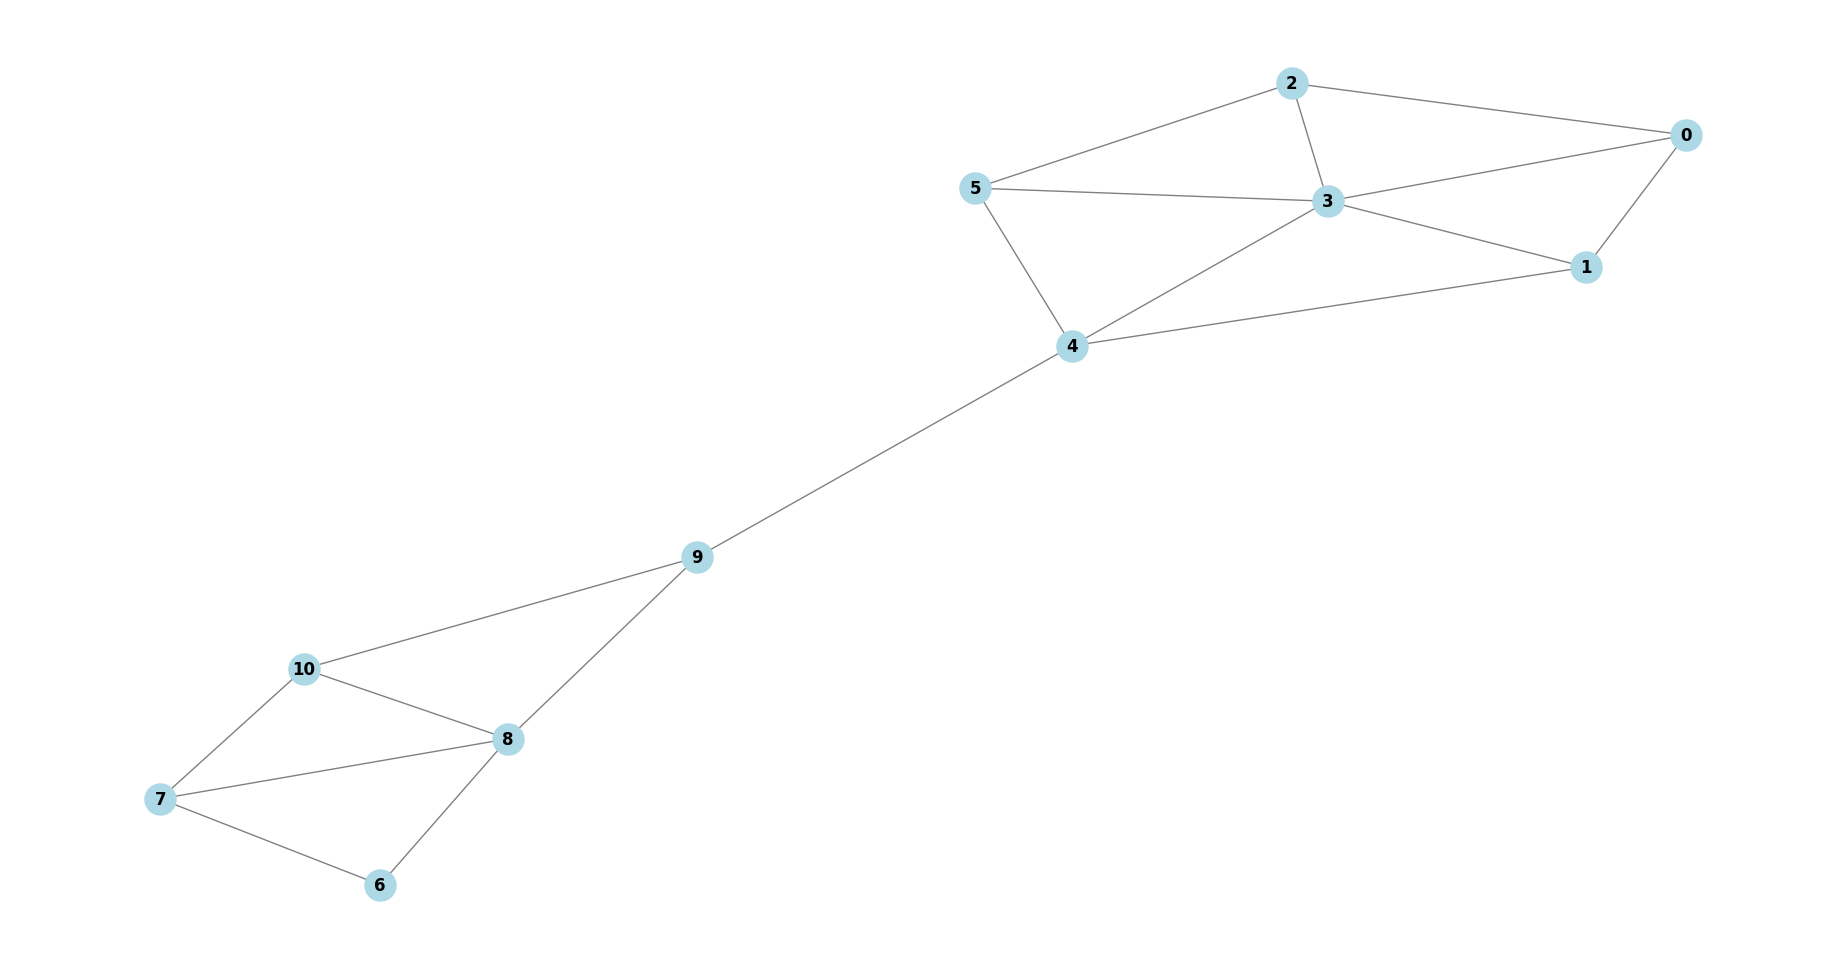
\includegraphics[width=0.6\textwidth]{congraph.png}
    \caption{A Connected Graph}
    \label{fig:ConnectedGraph}
\end{figure}

The eigenvalues for the Laplacian matrix from the above graph are: 0, 0.214, 1.81, 2.382, 2.655, 3.368, 4.441, 4.618, 4.94, 5.461, 6.11.

\subsection*{But here in this graph:}
\begin{figure}[h]
    \centering
    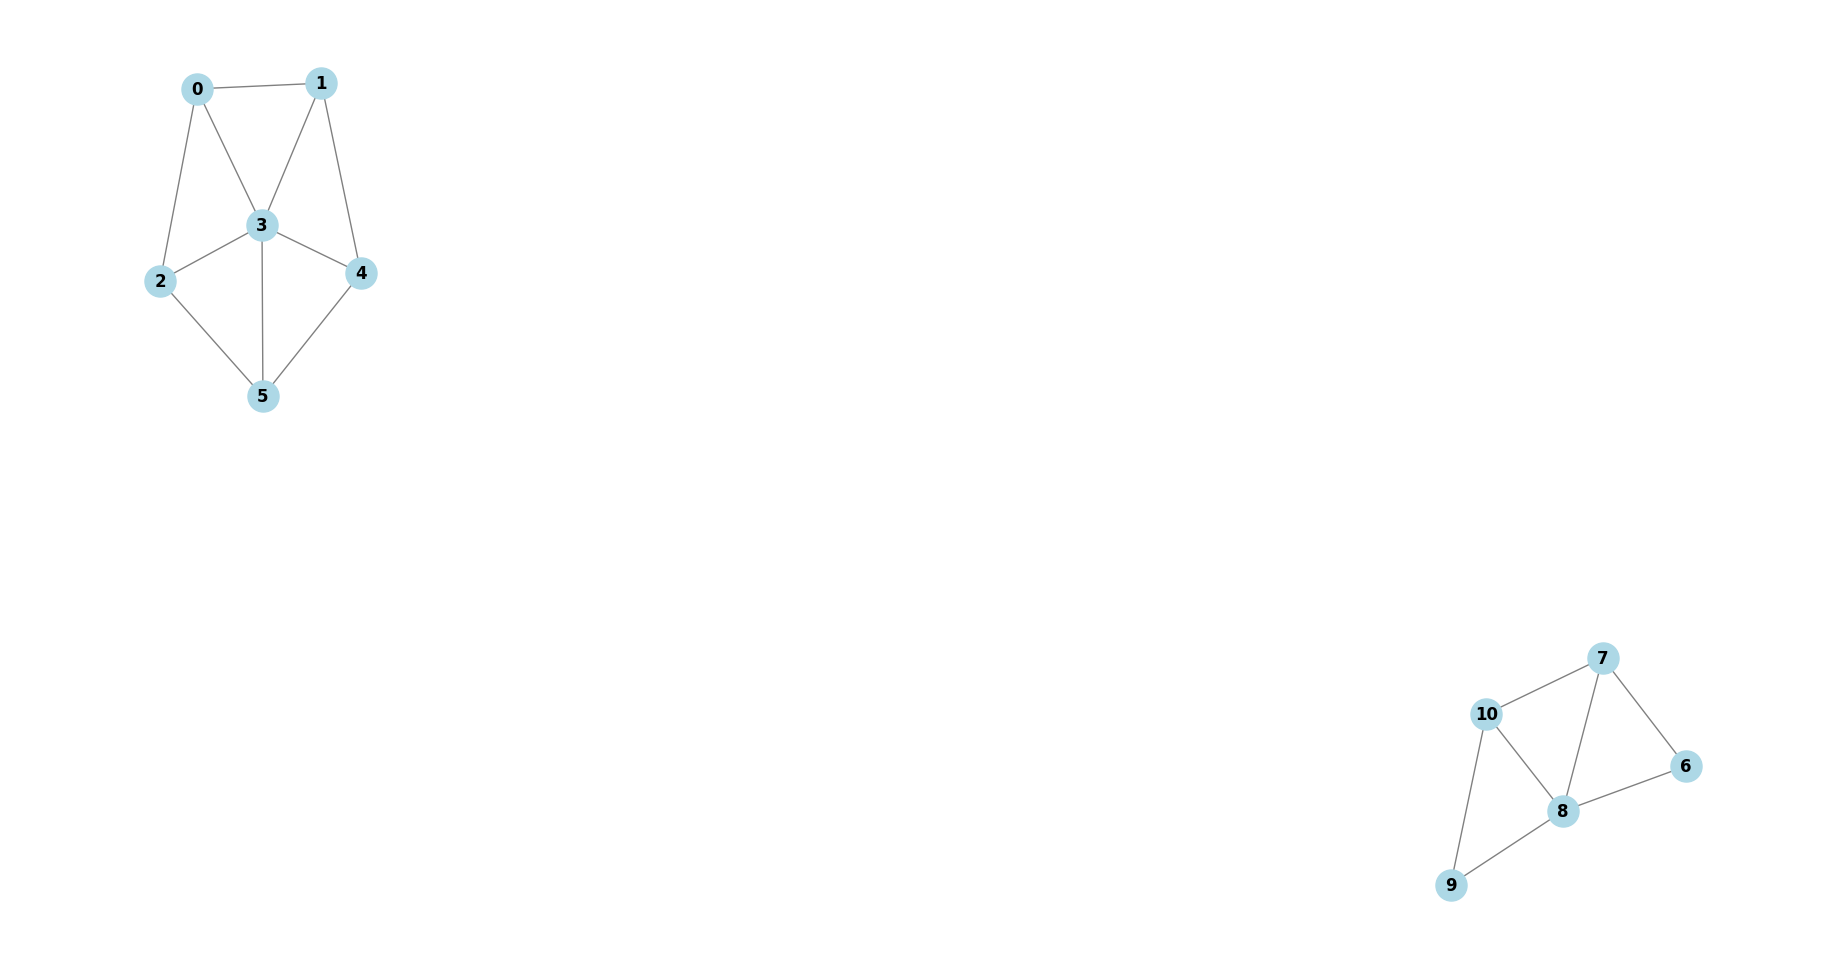
\includegraphics[width=0.6\textwidth]{discon.png}
    \caption{A Disconnected Graph}
    \label{fig:disConnectedGraph}
\end{figure}

The eigenvalues for the Laplacian matrix from the above graph are: 0, 0, 1.586, 2.382, 2.382, 3, 4.414, 4.618, 4.618, 5, 6.

From the above two examples, we can tell that a graph with the second lowest eigenvalue as 0 can be a disconnected graph.



\section*{Applications of Laplacian Matrix Eigenvalues}

\subsection*{Graph Partitioning}

The eigenvalues of the Laplacian matrix can be used in graph partitioning algorithms. These algorithms aim to divide a graph into multiple components or clusters based on the connectivity of the graph. The second smallest eigenvalue, being related to graph connectivity, can be utilized as a criterion for determining the quality of graph partitioning methods.

\subsection*{Spectral Graph Theory}

The Laplacian matrix and its eigenvalues play a significant role in spectral graph theory. Spectral graph theory studies the properties of graphs using linear algebraic techniques. The eigenvalues of the Laplacian matrix provide insights into the structure, connectivity, and properties of graphs. The theorem you mentioned is a fundamental result in spectral graph theory.

\subsection*{Network Analysis}

The theorem can be applied in the analysis of various networks, such as social networks, transportation networks, and communication networks. By examining the eigenvalues of the Laplacian matrix, particularly the second smallest eigenvalue, researchers can gain insights into the connectivity and structural properties of these networks.


\section*{Laplacian Eigen Values}
Laplacian eigenvalues, also known as Laplacian spectrum or Laplacian eigenfrequencies, are a set of mathematical properties associated with the Laplacian operator.

In the context of graph theory, the Laplacian eigenvalues are defined for a graph, which is a collection of vertices (nodes) connected by edges. The Laplacian matrix of a graph is a square matrix that encodes the graph's connectivity information. Each entry of the Laplacian matrix represents the connection between two vertices, with positive values indicating the presence of an edge and negative values representing the weights or conductance of the edges.

The eigenvalues of a Laplacian matrix provide valuable insights into the structure and properties of a graph. Here, I will elaborate on the characteristics associated with each eigenvalue of a Laplacian matrix.

\subsection*{Zero Eigenvalue}

One eigenvalue must equal to 0 for a graph:

\textbf{Proof:}

When we subtract the adjacency matrix from the degree matrix to form the Laplacian matrix, we can observe that the row sums of the resulting matrix are all zero. This property implies that the vector of all ones (a constant vector) is an eigenvector associated with the eigenvalue zero.

This zero eigenvalue and its corresponding eigenvector have important implications. It reflects that there is always a trivial solution to the Laplacian matrix equation, where the sum of values at each vertex is zero. This property corresponds to the graph being connected, as there is no isolated component or disconnected subgraph.

\subsection*{Classification of Laplacian Eigenvalues}

\textbf{Zero Eigenvalue:} As mentioned earlier, a Laplacian matrix always has a zero eigenvalue. It corresponds to a constant eigenvector, where all elements of the vector are the same. This eigenvalue signifies the connectivity of the graph and indicates that the graph is connected without any isolated components.

\textbf{Positive Eigenvalues:} The positive eigenvalues of the Laplacian matrix provide information about the connectivity and expansion properties of the graph. The magnitude of these eigenvalues indicates how fast information can spread or diffuse across the graph. Larger positive eigenvalues imply faster diffusion and better connectivity within the graph.

The sum of all positive eigenvalues corresponds to the sum of all degrees of the graph. This property is known as the "degree-sum theorem" and provides a useful relationship between the Laplacian eigenvalues and the graph's vertex degrees.

The first positive eigenvalue, often referred to as the "Fiedler eigenvalue," plays a crucial role in spectral graph theory. It divides the graph into two or more clusters based on the associated eigenvector. Spectral clustering algorithms utilize this eigenvalue to perform graph partitioning and clustering tasks.

\textbf{Negative Eigenvalues:} In some cases, the Laplacian matrix may have negative eigenvalues. The presence of negative eigenvalues indicates that the graph has a non-trivial bipartite structure or a sign of imbalance in the graph's connectivity.

The magnitude of negative eigenvalues provides information about the extent of the imbalance or bipartite structure within the graph. Larger negative eigenvalues suggest a stronger bipartite structure or imbalance.

It's important to note that the Laplacian matrix of a graph is always a symmetric and positive semi-definite matrix. Therefore, all the eigenvalues are real numbers, and they can be ordered from smallest to largest.

\textbf{Spectral Gap:} The difference between consecutive eigenvalues is referred to as the "spectral gap." The spectral gap provides insights into the connectivity and conductance properties of the graph. A larger spectral gap indicates a graph with stronger connectivity and better conductance between its components.

These are some additional aspects related to Laplacian eigenvalues. They offer a rich set of information about graph properties, connectivity, conductance, community structure, and even applications in graph drawing and random walks. By examining the Laplacian eigenvalues, we can gain insights into the underlying structure and behavior of graphs.

\section*{Uses:}

\textbf {Graph Partitioning and Clustering:} The Laplacian eigenvalues and eigenvectors are extensively employed in spectral graph partitioning and clustering algorithms. By analyzing the eigenvalues, particularly the second smallest eigenvalue (algebraic connectivity), and the corresponding eigenvector, the graph can be divided into clusters or partitions, revealing underlying community structures.

\textbf {Graph Drawing and Visualization:} Laplacian eigenvalues and eigenvectors are utilized in graph drawing and visualization techniques. They help determine the optimal layout of vertices in a graph, with connected vertices positioned close to each other and disconnected vertices positioned far apart. This aids in visualizing the graph's structure and relationships.

\textbf {Graph-based Image Segmentation:} Laplacian eigenvalues are utilized in image processing tasks, particularly image segmentation. The Laplacian matrix is constructed based on the image's graph representation, and the eigenvalues and eigenvectors of the Laplacian matrix assist in identifying distinct regions or objects within the image.

\textbf {Community Detection and Social Network Analysis:} Laplacian eigenvalues are employed in community detection algorithms in social network analysis. By analyzing the eigenvalues and eigenvectors of the Laplacian matrix, communities or groups of densely connected nodes can be identified in the network, revealing patterns and structures in the social system.

\textbf {Spectral Graph Theory:} Laplacian eigenvalues play a fundamental role in spectral graph theory, a branch of mathematics that investigates graph properties using the eigenvalues and eigenvectors of matrices associated with the graph. The Laplacian eigenvalues provide insights into graph connectivity, expansion, and symmetries.

\textbf {Random Walks on Graphs:} Laplacian eigenvalues are connected to random walks on graphs. The second smallest eigenvalue, known as the algebraic connectivity, and its associated eigenvector describe the behavior and convergence properties of random walks on the graph. This information is useful in studying diffusion processes and information propagation on networks.

\textbf {Machine Learning and Data Analysis:} Laplacian eigenvalues have found applications in machine learning and data analysis tasks. They are used in dimensionality reduction techniques like Laplacian eigenmaps and spectral embedding, where the eigenvalues and eigenvectors of the Laplacian matrix are employed to transform high-dimensional data into a lower-dimensional representation while preserving the underlying structure.

\textbf {Network Resilience and Robustness:} The Laplacian eigenvalues provide insights into the resilience and robustness of networks. Large eigenvalues indicate strong connectivity and faster information diffusion, while the spectral gap between eigenvalues reveals the network's vulnerability to perturbations and structural changes.

\end{document}

